\documentclass[../m082main.tex]{subfiles}
\graphicspath{{\subfix{../figures/}}}

\begin{document}

\chapter{Systems of Differential Equations}

\section{Introduction}
\medskip
\begin{definition}[System of differential equations]
    A system of differential equations has the general form
    \[ \mbf{x}'(t) = \mbf{f}(t, \mbf{x}(t)). \]
    In terms of components, this is
    \begin{align*}
        x_1'(t) &= f_1 (t, x_1(t), x_2(t), \ldots, x_n(t)) \\
        &\;\;\vdots \\
        x_n'(t) &= f_n (t, x_1(t), x_2(t), \ldots, x_n(t))
    \end{align*}
    Here, the state vector $\mbf{x}(t)$ denotes the states (or quantities) of interest, $\mbf{x}'(t)$ denotes the rates of change of the states, and $\mbf{f}(t, \mbf{x}(t))$ represents the governing dynamics that describe how the states change over time in response to interactions among the states or external forces.
\end{definition}

Not only do systems of DEs allow us to consider different types of problems than those we've seen so far, but they allow us to look at familiar problems through a different lens: any ``scalar'' differential equation can be written as a system of first-order differential equations.
For example, consider the $n$th-order DE
\[ \frac{d^{n}y}{dt^{n}} = f(t, y, y', \ldots, y^{(n-1)}). \]
If we define state variables $x_1 = y,\; x_2 = y',\; \ldots,\; x_n = y^{(n-1)}$, we can recast the DE as the system
\begin{align*}
    x_1' &= x_2 \\
    x_2' &= x_3 \\
    &\;\;\vdots \\
    x_{n-1}' &= x_n \\
    x_n' &= f(t, x_1, x_2, \ldots, x_n)
\end{align*}
Now, we'll extend some familiar terminology to these new problems.

\begin{definition}[Linear system of DEs]
    A system of differential equations $\mbf{x}' = \mbf{f}(t, \mbf{x})$ is linear if each component of $\mbf{f}$ depends linearly on the state variables.
    Otherwise, it is nonlinear.
\end{definition}

\begin{definition}[Autonomous system of DEs]
    A system of differential equations $\mbf{x}' = \mbf{f}(t, \mbf{x})$ is autonomous if $\mbf{f}$ does not depend explicitly on the variable $t$, that is, if $\partial f / \partial t = \mbf{0}$.
    Otherwise, it is nonautonomous.
\end{definition}

Note that any nonautonomous system can be recast as an autonomous one by defining a new state variable for the independent variable.
We thus restrict our attention to autonomous systems without loss of generality.

\begin{definition}[Equilibrium points of a system of DEs]
    A point $\mbf{x}_0$ is an equilibrium point of the system $\mbf{x}' = \mbf{f}(\mbf{x})$ if $\mbf{f}(\mbf{x}_0) = \mbf{0}$.
\end{definition}

Finally, we give a condition for whether a solution to a system exists.
It is an extension of Theorem 2.3.

\begin{theorem}[Existence and uniqueness of solutions]
    Let $\mbf{f}(x)$ have components $f_1, f_2, \ldots, f_n$.
    If $f_i$ and $\partial f_i / \partial x_j$ ($1 \leq i,j \leq n$) are continuous in a neighborhood of $\mbf{x}_0$ then there exists $\varepsilon > 0$ such that the initial-value problem
    \[ \mbf{x}' = \mbf{f}(\mbf{x}), \quad \mbf{x}(t_0) = \mbf{x}_0. \]
    has a unique solution $\mbf{x}(t)$, defined for $t \in (t_0 - \varepsilon, t_0 + \varepsilon)$.
\end{theorem}

\section{Constant-Coefficient Linear Systems}
\subsection{Fundamental Matrices and the Flow}
For now, we'll focus our attention on homogeneous constant-coefficient linear systems.
These can be written in the form $\mbf{x}' = A \mbf{x}$, where $A$ is an $n \times n$ matrix and $\mbf{x} : \R \to \R^n$.
We first verify that this problem can be solved for any initial condition.

\begin{theorem}[Global solution theorem]
    Let $A$ be an $n \times n$ matrix with real entries.
    For each $\mbf{x}_0 \in \R^n$ the initial-value problem
    \[ \mbf{x}' = A\mbf{x}, \quad \mbf{x}(t_0) = \mbf{x}_0. \]
    has a unique solution $\mbf{x}(t)$ which is defined for all $t \in (-\infty, \infty)$.
\end{theorem}

This gives us some information about the general solution to a differential equation of this form.

\begin{corollary}[Solutions as a vector space]
    The set of solutions to $\mbf{x}' = A \mbf{x}$ is an $n$-dimensional vector space.
\end{corollary}

Therefore, the general solution of $\mbf{x}' = A \mbf{x}$ has the form
\[ \mbf{x}(t) = c_1 \mbf{x}_1(t) + c_2 \mbf{x}_2 + \cdots + c_n \mbf{x}_n (t) = \begin{bmatrix} | & | &  & | \\ \mbf{x}_1(x) & \mbf{x}_2(x) & \cdots & \mbf{x}_n(t) \\ | & | &  & | \end{bmatrix} \begin{bmatrix} c_1 \\ c_2 \\ \vdots \\ c_n \end{bmatrix} \]
where $\mbf{x}_1, \mbf{x}_2, \ldots, \mbf{x}_n$ are linearly independent solutions and $c_i$ are arbitrary constants.

The matrix of linearly independent solution vectors is important enough to warrant a definition.

\begin{definition}[Fundamental matrix]
    A fundamental matrix $\Psi (t)$ of the system $\mbf{x}' = A \mbf{x}$ is one whose columns are linearly independent solutions of the system.
\end{definition}

There's a couple of ways we can go about finding a fundamental matrix.
The first involves making an ansatz: based on results from Section 3.2, we might guess that a particular solution to the system is some vector of exponentials, say $\mbf{x}(t) = e^{\lambda t} \mbf{v}$ for a constant vector $\mbf{v}$.
To determine $\lambda$ and $\mbf{v}$, consider how $\mbf{x}$ is a solution to the system of DEs if and only if
\begin{align*}
    \mbf{x}' &= A \mbf{x} \\
    \lambda e^{\lambda t} \mbf{v} &= A (e^{\lambda t} \mbf{v}) \\
    \lambda \mbf{v} &= A \mbf{v}
\end{align*}
We can see, now, that $\lambda$ and $\mbf{v}$ comprise an eigenvalue-eigenvector pair (an ``eigenpair'') of $A$.
We formalize this in a theorem.

\begin{theorem}[Solution to a diagonalizable linear system]
    Let $A$ be a diagonalizable $n \times n$ matrix with eigenvalues $\lambda_1, \lambda_2, \ldots, \lambda_n$ and corresponding eigenvectors $\mbf{v}_1, \mbf{v}_2, \ldots, \mbf{v}_n$.
    The general solution to the system $\mbf{x}' = A \mbf{x}$ is
    \[ \mbf{x}(t) = c_1 e^{\lambda_1 t} \mbf{v}_1 + c_2e^{\lambda_2 t} \mbf{v}_2 + \cdots + c_n e^{\lambda_n t} \mbf{v}_n, \]
    where $c_1, c_2, \ldots, c_n$ are constants.
\end{theorem}

Thus, so long as $A$ is diagonalizable (has $n$ distinct eigenvectors), computing the eigendata of $A$ gives us sufficient information to determine $n$ linearly independent solutions to the system, giving us the general solution $\mbf{x}(t) = \Psi (t) \mbf{c}$.
It doesn't matter if we get repeated eigenvalues---linearly independent eigenvectors give linearly independent solutions.

As a side note, if we have complex eigenvalues, we can use the following shortcut to get two linearly independent solutions.

\begin{theorem}[Linearly independent solutions from complex eigendata]
    Let $\mbf{x}(t) = e^{\lambda t} \mbf{v}$, $\lambda \in \C$ solve the system $\mbf{x}' = A \mbf{x}$.
    Define $\lambda = \alpha + i\beta$ and $\mbf{v} = \mbf{p} + i\mbf{q}$.
    Then $\pfn{Re} (\mbf{x}(t))$ and $\pfn{Im} (\mbf{x}(t))$ are linearly independent solutions to the system, with
    \begin{align*}
        \pfn{Re}(\mbf{x}(t)) &= e^{\alpha t} (\cos \beta t \; \mbf{p} - \sin \beta t \; \mbf{q}) \\
        \pfn{Im}(\mbf{x}(t)) &= e^{\alpha t} (\sin \beta t \; \mbf{p} + \cos \beta t \; \mbf{q})
    \end{align*}
\end{theorem}

Now, if we are given initial conditions, we can use $\Psi$ to find the solution to the IVP without going through all the trouble of solving a system of equations.
If $\mbf{x}(0) = \mbf{x}_0$, then we must have $\Psi (0) \mbf{c} = \mbf{x}_0$.
Solving for $\mbf{c}$ gives $\mbf{c} = \Psi^{-1}(0) \mbf{x}_0$.
Therefore, the solution to the IVP is
\[ \mbf{x}(t) = \Psi(t) \Psi^{-1}(0) \mbf{x}_0. \]
The matrix $\Psi(t) \Psi^{-1}(0)$ is the key to understanding linear systems and the global behavior of their solutions.
It is so important that it gets its own name.

\begin{definition}[Flow of a linear system]
    The flow of the linear system $\mbf{x}' = A \mbf{x}$ is the matrix $\Psi(t) \Psi^{-1}(0)$, where $\Psi$ is any fundamental matrix.
\end{definition}

All this information is great, but again, we can only get it if $A$ is diagonalizable.
If this is not the case, we must resort to other means.

\subsection{Matrix Exponentials}
First, notice that the initial-value problem $\mbf{x}' = \mbf{f}(\mbf{x})$, $\mbf{x}(0) = \mbf{x}_0$, is equivalent to the integral equation
\[ \mbf{x}(t) = \mbf{x}_0 + \int_0^t \mbf{f}(\mbf{x}(s))\;ds. \]
Like many differential equations, it will not always be possible to solve this integral equation directly, but we can approximate a solution.
One method of doing so is defined below.

\begin{theorem}[Picard iteration]
    Consider the IVP $\mbf{x}' = \mbf{f}(\mbf{x})$, $\mbf{x}(0) = \mbf{x}_0$.
    Let $\mbf{x}_0(t) = \mbf{x}_0$ and for $n \in \N$ define $\mbf{x}_n$ by
    \[ \mbf{x}_n(t) = \mbf{x}_0 + \int_0^t \mbf{f}(\mbf{x}_{n-1}(s))\;ds. \]
    If the approximate solutions $\mbf{x}_n$ converge to some function $\mbf{x}$, then the limit function $\mbf{x}$ is the unique solution to the IVP.
\end{theorem}

Picard iteration gives us a concrete way to approximate solutions to first-order systems.
Further, if we can determine the limit of $\mbf{x}_n$, we can use it to solve the first-order system outright.
We'll do this below.

\begin{example}[Solving a linear system using Picard iteration]
    Our aim is to solve the initial-value problem $\mbf{x}' = A \mbf{x}$, $\mbf{x}(0) = \mbf{x}_0$.
    The Picard iterates are defined by
    \begin{align*}
        \mbf{x}_n(t) &= \mbf{x}_0 + \int_0^t A \mbf{x}_{n-1}(s) \;ds \\
        \mbf{x}_n(t) &= \mbf{x}_0 + A \int_0^t \mbf{x}_{n-1}(s) \;ds
    \end{align*}
    After we go through some iterations, we find that the iterates converge to the exponential power series
    \[ \mbf{x}(t) = \left[ I + At + \frac{A^2t^2}{2!} + \cdots + \frac{A^nt^n}{n!} + \cdots \right] \mbf{x_0}. \]
    So, this is the solution to the IVP and we will use it to define a new matrix operation.
\end{example}

\begin{definition}[Matrix exponential]
    If $A$ is a square matrix, we define its matrix exponential as
    \[ e^{A} = \sum_{k = 0}^\infty \frac{A^{k}}{k!} = I + A + \frac{A^2}{2!} + \frac{A^3}{3!} + \cdots. \]
\end{definition}

\begin{theorem}[Solution to a homogeneous linear system]
    The solution to the IVP $\mbf{x}' = A \mbf{x}$, $\mbf{x}(0) = \mbf{x}_0$ is
    \[ \mbf{x}(t) = e^{At} \mbf{x}_0. \]
\end{theorem}

We can compute some matrix exponentials simply using the power series definition, but this can get a bit tedious.
We'll give a few useful properties that can make computing matrix exponentials a little easier.

\begin{theorem}[Selected matrix exponentials]
    \begin{enumerate}[label=(\alph*)]
        \item Let $A$ be a diagonal matrix with diagonal entries $\lambda_1, \lambda_2, \ldots, \lambda_n$.
        Then its matrix exponential is also diagonal, with
        \[ e^{A} = \begin{bmatrix} e^{\lambda_1} & 0 & \cdots & 0 \\ 0 & e^{\lambda_2} & \cdots & 0 \\ \vdots & \vdots & \ddots & \vdots \\ 0 & 0 & \cdots & e^{\lambda_n} \end{bmatrix}. \]
        \item Let $M = \begin{bmatrix} 0 & q \\ -q & 0 \end{bmatrix}$ where $q > 0$ is a constant.
        Then its matrix exponential is
        \[ e^{Mt} = \begin{bmatrix} \cos qt & \sin qt \\ -\sin qt & \cos qt \end{bmatrix}. \]
    \end{enumerate}
\end{theorem}

\begin{theorem}[Condition for commutative exponentials]
    Let $A$ and $B$ be square matrices of the same size.
    Then the following statements are equivalent.
    \begin{enumerate}[label=(\alph*)]
        \item $A$ and $B$ commute.
        \item $e^{A + B} = e^{A} e^{B}$.
        \item $e^{A} e^{B} = e^{B} e^{A}$.
    \end{enumerate}
\end{theorem}

So we've found two ways to represent the solution to the IVP: $\mbf{x}(t) = \Psi(t) \Psi^{-1}(0)\mbf{x}_0$ and $\mbf{x}(t) = e^{At} \mbf{x}_0$.
However, we've seen that the solution to an IVP is unique, giving us the following.

\begin{theorem}[Characterization of $e^{At}$]
    Let $\Psi$ be any fundamental matrix of the linear system $\mbf{x}' = A\mbf{x}$.
    Then
    \[ e^{At} = \Psi (t) \Psi^{-1} (0). \]
\end{theorem}

We now have two ways to compute the flow of $\mbf{x}' = A \mbf{x}$: using the fundamental matrix and via the power series definition of the matrix exponential.
One final way involves the diagonalization of $A$, made practical by the following theorem.

\begin{theorem}[Similarity of matrix exponentials]
    If $B = P^{-1} A P$, then $e^{Bt} = P^{-1} e^{At} P$.
\end{theorem}

So, similar to how we compute powers of matrices like $A^{10}$, we can compute matrix exponentials by diagonalizing $A$, computing the exponential, and then undoing the diagonalization to find $e^{At}$.

\subsection{Inhomogeneous Systems}
The matrix exponential gives us an important insight into how to solve linear systems with a forcing term.
Key to this insight is that the derivative of a matrix exponential is analogous to that of a scalar exponential.

\begin{lemma}[Derivative of a matrix exponential]
    If $A \in M_n (\R)$, then $\dfrac{d}{dt} \left[ e^{At} \right] = A e^{At} = e^{At} A$.
\end{lemma}

Now we can solve the general constant-coefficient linear system $\mbf{x}' = A \mbf{x} + \mbf{F}(t)$.

\begin{example}[Solving a forced constant-coefficient linear system]
    We aim to find the general solution to the initial-value problem
    \[ \mbf{x}' = A \mbf{x} + \mbf{F}, \quad \mbf{x}(0) = \mbf{x}_0. \]
    Taking inspiration from the integrating factor method discussed early in the course, we rewrite the system as
    \[ \mbf{x}' - A \mbf{x} = \mbf{F} \]
    and multiply by the integrating factor $\mu(t) = e^{\int (-A) dt} = e^{-A t}$ to get
    \begin{align*}
        e^{-At} \mbf{x}' - e^{-At} A \mbf{x} &= e^{-At} \mbf{F} \\
        \frac{d}{dt} \left[ e^{-At} \mbf{x} \right] &= e^{-At} \mbf{F} \\
        e^{-At}\mbf{x} - \mbf{x}_0 &= \int_{0}^{t} e^{-As} \mbf{F} \;ds \\
        \mbf{x}(t) &= e^{At} \mbf{x}_0 + e^{At} \int_0^t e^{-As} \mbf{F} \;ds
    \end{align*}
    This is the solution to the IVP.
\end{example}

\begin{theorem}[Solution to an inhomogeneous linear system]
    The unique solution of the inhomogeneous system $\mbf{x}' = A \mbf{x} + F$ with initial value $\mbf{x}(0) = \mbf{x}_0$ is
    \[ \mbf{x}(t) = e^{At} \mbf{x}_0 + e^{At} \int_0^t e^{-As} \mbf{F}(s) \;ds. \]
    Written in terms of a fundamental matrix $\Psi$,
    \[ \mbf{x}(t) = \Psi(t) \Psi^{-1}(0) \mbf{x}_0 + \Psi(t) \int_0^t \Psi^{-1}(s) \mbf{F}(s) \;ds. \]
\end{theorem}

Notice how this solution can be interpreted as the sum of a homogeneous solution $\mbf{x}_h$ and a particular one $\mbf{x}_p$.
$\mbf{x}_h$ is the system's response to the initial conditions, and $\mbf{x}_p$ is the cumulative response to the forcing.

\subsection{Phase Portraits}
Here, we'll develop a way to visualize the dynamics of two-dimensional systems.
This can be directly extended to three dimensions and, more abstractly, higher dimensions.
We begin with a connection between the eigendata of $A$ and $e^{At}$.

\begin{theorem}[Eigendata of a matrix exponential]
    If $(\lambda, \mbf{v})$ is an eigenpair of $A$, then $(e^{\lambda t}, \mbf{v})$ is an eigenpair of $e^{At}$.
\end{theorem}

If $A$ is diagonalizable, then any initial condition $\mbf{x}_0$ can be written as a linear combination of the eigenvectors of $A$.
So when $e^{At}$ acts on $\mbf{x}_0$, the matrix has the effect of scaling the eigen-components of $\mbf{x}_0$ exponentially in $t$.
The nature of this scaling, determined by the eigenvalues of $A$, entirely determines the path a solution curve will take with increasing time.
When several of these paths are compiled together, we get a good picture of how the flow acts on state space.

\begin{definition}[Phase portrait]
    A phase portrait is a diagram in state space that indicates several solution curves (also called orbits or trajectories).
    The solution curves are flow lines of the vector field $\mbf{f}(\mbf{x})$ since $\mbf{f}'(t) = \mbf{f}(\mbf{x}()t)$.
\end{definition}

Key to predicting what the orbits will look like is the distinction between the real and complex parts of an eigenvalue $\lambda$.

The real part of $\lambda$ controls the exponential growth or decay of a system.
\begin{itemize}
    \item If $\pfn{Re} (\lambda) > 0$, then the system exhibits growth.
    \item If $\pfn{Re} (\lambda) < 0$, then the system exhibits decay.
    \item If $\pfn{Re} (\lambda) = 0$, then we get neither growth nor decay, so the ``magnitude'' of the system remains constant.
\end{itemize}
If the system has two real eigenvalues, then the scaling described here happens in the direction of each eigenvalue's corresponding eigenvector.

The imaginary part of $\lambda$ controls the rotation of a system.
\begin{itemize}
    \item If $\pfn{Im} (\lambda) > 0$, then the system rotates counterclockwise.
    \item If $\pfn{Im} (\lambda) < 0$, then the system rotates clockwise.
    \item If $\pfn{Im} (\lambda) = 0$, then the system does not rotate.
\end{itemize}

Now, using the fact that
\[ \lambda_{1,2} = \frac{\pfn{tr} A \pm \sqrt{(\pfn{tr} A)^2 - 4 \det A}}{2}, \]
we can graphically represent all possible phase portraits.
The figure below is courtesy of Prof. Jacobsen.
\begin{center}
    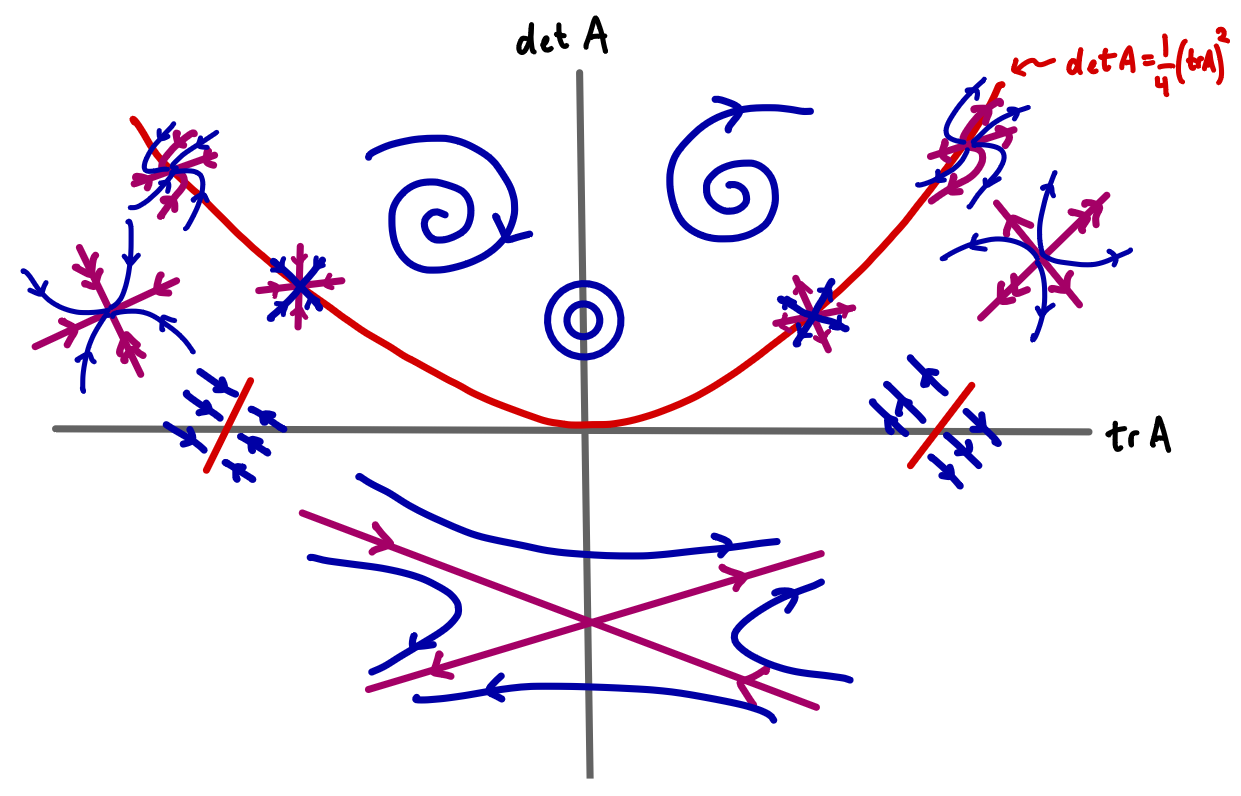
\includegraphics[width=0.65\textwidth]{zoology.png}
\end{center}
Each portion of the diagram above represents a different class of phase portrait.
A few of these have special names, which are given in the chart below.
\begin{center}
    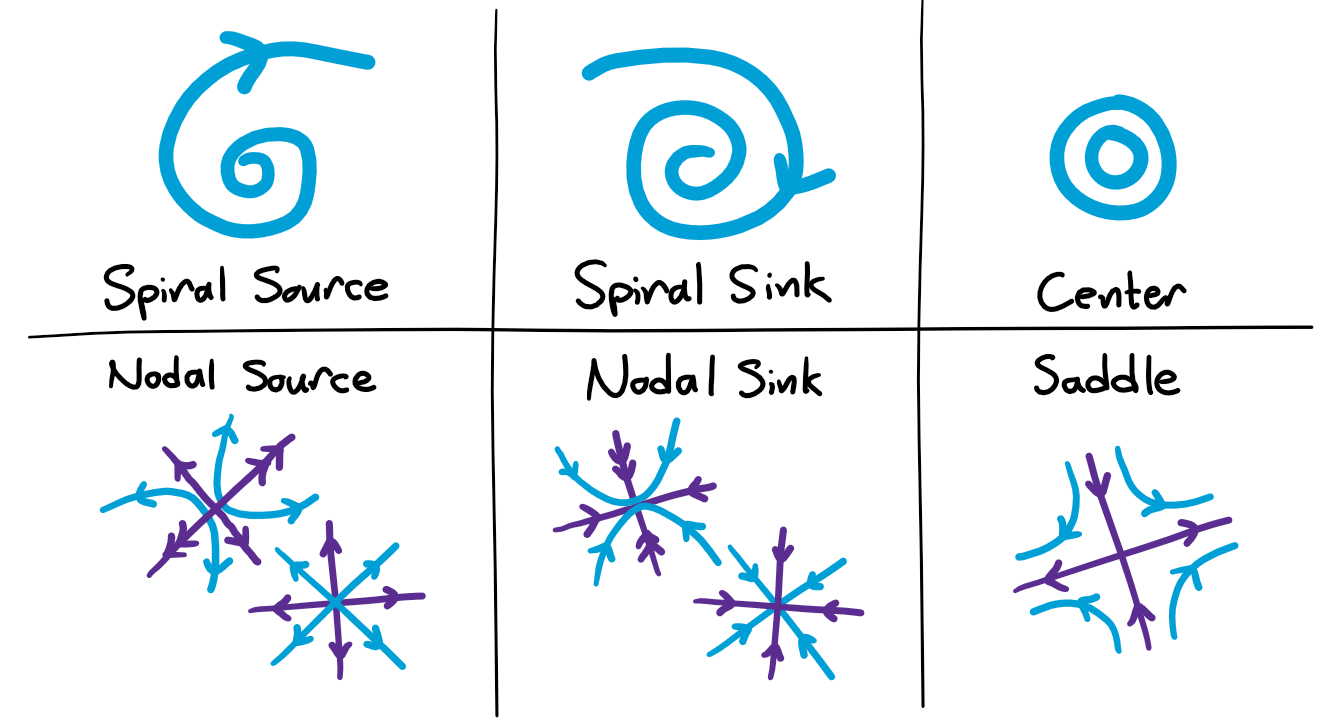
\includegraphics[width=0.75\textwidth]{zoologyClassification.png}
\end{center}

There is a variety of definitive statements we can make about the behavior of initial conditions under the influence of each of these flows.
We'll give one of these to finish off our discussion of linear systems.

\begin{theorem}[Asymptotic stability theorem]
    If $\pfn{Re} (\lambda) < 0$ for all eigenvalues $\lambda$ of $A$, then all solutions of $\mbf{x}' = A \mbf{x}$ satisfy $\mbf{x}(t) \to \mbf{0}$ as $t \to \infty$.
\end{theorem}

\section{Nonlinear Systems}
\subsection{Local Linearization}
In general, nonlinear systems are much more difficult to work with than linear ones.
None of the nice linear structure we developed in the previous section applies anymore, and in fact exact analytic formulas for solutions rarely exist.

A quick examination of a nonlinear phase portrait shows that nonlinear systems can have multiple isolated equilibrium points.
This is in direct contrast to linear phase portraits, which have exactly one equilibrium point at the origin.
These equilibria, however, are not too different form those found in linear systems; in fact, one important method of analyzing nonlinear systems is to exploit the fact that equilibria are locally linear.

To linearize an equilibrium, we apply the change of coordinates $\mbf{u}(t) = \mbf{x}(t) - \mbf{x}_0$ and analyze the dynamics of $\mbf{u}$ when it is sufficiently small.
We know that
\begin{align*}
    \mbf{u}' &= \mbf{x}'= \mbf{f} (\mbf{x}) \\
    &= \mbf{f} (\mbf{x}_0 + \mbf{u}) \\
    &= \mbf{f} (\mbf{x}_0) + D \mbf{f} (\mbf{x}_0) \mbf{u} + \mathcal{O} (\|\mbf{u}\|^2)
\end{align*}
where $D \mbf{f} (\mbf{x}_0)$ is the matrix whose $(i,j)$ entry is the partial derivative of $f_i$ with respect to $x_j$.
(This is called the Jacobian matrix.)
The higher-order terms disappear, and since $\mbf{x}_0$ is an equilibrium point we know that $\mbf{f}(\mbf{x}_0)$.
This gives us the following result.

\begin{theorem}[Local linearization]
    The linearization of $\mbf{x}'= \mbf{f} (\mbf{x})$ at the equilibrium point $\mbf{x}_0$ is the linear system
    \[ \mbf{u}' = A \mbf{u} \]
    where $\mbf{u}(t) = \mbf{x}(t) - \mbf{x}_0$ and
    \[ A = D \mbf{f} (\mbf{x}_0), \]
    the derivative matrix of $\mbf{f}$ evaluated at $\mbf{x}_0$.
\end{theorem}

Using this, we can classify each equilibrium point of a system by stability.

\begin{definition}[Equilibrium stability]
    An equilibrium point is stable if $\pfn{Re} (\lambda) \leq 0$ for all eigenvalues $\lambda$ of $A = D \mbf{f} (\mbf{x}_0)$.
    An equilibrium point is asymptotically stable if $\pfn{Re} < 0$ for all eigenvalues $\lambda$ of $A = D \mbf{f} (\mbf{x}_0)$.
    Otherwise we ssy the equilibrium point is unstable.
\end{definition}

Informally:
\begin{itemize}
    \item A stable equilibrium point is one where starts that start close will stay close for all future time.
    \item An asymptotically stable equilibrium point is on where states that start close will asymptotically converge back to the equilibrium point as time increases.
    \item An unstable equilibrium point is where where there are states that start close but do not stay close.
\end{itemize}
In most cases, a system's linearization gives us an accurate understanding of how the system will behave near an equilibrium point.
However, this won't always be true; a condition for this is below.

\begin{theorem}[Hartman-Grobman theorem]
    If $\mbf{x}_0$ is an equilibrium point of $\mbf{x}'= \mbf{f}(\mbf{x})$ and $\pfn{Re} (\lambda) \neq 0$ for all eigenvalues $\lambda$ of $D \mbf{f} (\mbf{x}_0)$, then the linearization at $\mbf{x}_0$ is ``faithful.''
\end{theorem}

This theorem can be used to prove a version of Theorem 4.15 for nonlinear systems.

\begin{theorem}[Local stability theorem]
    If $\mbf{x}_0$ is an equilibrium point of $\mbf{x}' = \mbf{f} (\mbf{x})$ and $\pfn{Re} < 0$ for all eigenvalues $\lambda$ of $D \mbf{f} (\mbf{x}_0)$, then all solutions that start sufficiently close to $\mbf{x}_0$ will satisfy $\mbf{x}(t) \to \mbf{x}_0$ and $t \to \infty$.
\end{theorem}

\subsection{Nullclines and Energy}
Linearization is not the only tool we can use to analyze nonlinear systems.

\begin{definition}[Nullclines]
    Consider the general system
    \begin{align*}
        \dot x &= f(x,y) \\
        \dot y &= g(x,y)
    \end{align*}
    The $x$-nullclines are defined by the equation $f(x,y) = 0$.
    The $y$-nullclines are defined by the equation $g(x,y) = 0$.
\end{definition}

Plotting the nullclines and drawing arrows on them to indicate the direction of the flow can be a striking way to roughly visualize the system's phase portrait, mainly rotation.

We can also make the observation that phase portraits look like level curve plots, with each solution curve representing a different level curve of some function.
In this way, each solution corresponds to some ``energy,'' and this energy is constant (conserved) over the entire solution curve.

\begin{definition}[Conserved quantity]
    A function $E : \R^n \to \R$ is a conserved quantity for $\mbf{x}' = \mbf{f} (\mbf{x})$ if
    \[ \frac{d}{dt} E (\mbf{x} (t)) = 0 \]
    for all solutions $\mbf{x} (t)$.
    (We also call $E$ an energy or constant of motion.)
    A system with a conserved quantity is called a conservative system.

    \textit{Note: We also assume $E$ is non-constant on any ball of radius $r$, because otherwise damped systems could have conserved quantities.}
\end{definition}

To show that a given quantity $E$ is conserved, we may simply compute the time derivative of $E$ and show that it is identically zero.
To find a conserved quantity, however, is an inverse problem---we may solve the DE $\dfrac{dy}{dx} = \dfrac{\dot y}{\dot x}$ to determine the level curves, rely on physical intuition, or use some other insights.

If we determine that the energy of a system is not conserved, it can give us important information about the stability of an equilibrium.

We can also use this energy view to warp state space in different ways that clarify which solution curves correspond to higher energies.

\subsection{Limit Cycles}
We'll finish off our discussion of systems by discussing a new type of solution that only appears in nonlinear systems.

\begin{definition}[Limit cycle]
    A limit cycle is an isolated periodic solution to a system of DEs.
\end{definition}

The key word here is ``isolated.''
This means that, given some limit cycle, there are no other limit cycles in its neighborhood.
This is in contrast with centers, in which there is a continuum of periodic solutions.

Given some linear system $\mbf{x}' = \mbf{f} (\mbf{x})$, in order to show that a limit cycle exists we must show that $f$ has a trapping region.
This is defined below.

\begin{definition}[Trapping region]
    A region of a vector field $\Omega$ is called a trapping region if the vector field points inward everywhere along the boundary $\partial \Omega$.
\end{definition}

If a solution curve enters a trapping region, there is no way to move radially inward or outward, because it will simply be deflected back.
However, there is no guarantee that it will lead to a limit cycle; we give a condition for this below.

\begin{theorem}[Poincaré-Bendixon theorem]
    If $\Omega$ is a trapping region for the planar system $\mbf{x}' = \mbf{f}(\mbf{x})$, $\mbf{x} \in \R^2$ and $\Omega$ contains no equilibrium points, then $\Omega$ contains at least one periodic solution.
\end{theorem}

If the periodic solutions in this trapping region are isolated, then they are limit cycles.

\end{document}